\documentclass[12pt]{article}
\usepackage{amsthm,amssymb,amsmath,amsfonts}
\usepackage[a4paper, top=25mm, bottom=30mm, left=25mm, right=25mm]{geometry}
\usepackage[pagebackref=false,colorlinks,linkcolor=black,citecolor=black]{hyperref}
\usepackage[nameinlink]{cleveref}
 \AtBeginDocument{%
    \crefname{equation}{برابری}{equations}%
    \crefname{chapter}{فصل}{chapters}%
    \crefname{section}{بخش}{sections}%
    \crefname{appendix}{پیوست}{appendices}%
    \crefname{enumi}{مورد}{items}%
    \crefname{footnote}{زیرنویس}{footnotes}%
    \crefname{figure}{شکل}{figures}%
    \crefname{table}{جدول}{tables}%
    \crefname{theorem}{قضیه}{theorems}%
    \crefname{lemma}{لم}{lemmas}%
    \crefname{corollary}{نتیجه}{corollaries}%
    \crefname{proposition}{گزاره}{propositions}%
    \crefname{definition}{تعریف}{definitions}%
    \crefname{result}{نتیجه}{results}%
    \crefname{example}{مثال}{examples}%
    \crefname{remark}{نکته}{remarks}%
    \crefname{note}{یادداشت}{notes}%
    \crefname{observation}{مشاهده}{observations}%
    \crefname{algorithm}{الگوریتم}{algorithms}%
    \crefname{cproof}{برهان}{cproofs}%
}

\usepackage{tikz}
\usepackage{graphicx}
\usepackage{booktabs}
\usepackage{color}
\usepackage{graphicx}
\usepackage{subcaption}

\usepackage{setspace}
\doublespacing

\usepackage{titletoc}
\usepackage{tocloft}
\usepackage{enumitem}
\usepackage{amsmath, amssymb}
\usepackage{algorithm}
\usepackage[noend]{algorithmic}
\renewcommand{\algorithmicrequire}{\textbf{Input:}}
\renewcommand{\algorithmicensure}{\textbf{Output:}}

\usepackage{tabularx}
\makeatletter
\newcommand{\multiline}[1]{%
  \begin{tabularx}{\dimexpr\linewidth-\ALG@thistlm}[t]{@{}X@{}}
    #1
  \end{tabularx}
}
\makeatother

\usepackage{float}
\usepackage{verbatim}
\makeindex
\usepackage{sectsty}
\usepackage{xepersian}
\SepMark{-}
\settextfont[Scale=1.2,Path=fonts/,BoldFont=B Nazanin Bold.ttf]{B Nazanin.ttf}
\setlatintextfont{Times New Roman}
\renewcommand{\labelitemi}{$\bullet$}

\theoremstyle{definition}
\newtheorem{definition}{تعریف}[section]
\newtheorem{remark}[definition]{نکته}
\newtheorem{note}[definition]{یادداشت}
\newtheorem{example}[definition]{نمونه}
\newtheorem{question}[definition]{سوال}
\newtheorem{remember}[definition]{یاداوری}
\newtheorem{observation}[definition]{مشاهده}
\theoremstyle{theorem}
\newtheorem{theorem}[definition]{قضیه}
\newtheorem{lemma}[definition]{لم}
\newtheorem{proposition}[definition]{گزاره}
\newtheorem{corollary}[definition]{نتیجه}
\newtheorem*{cproof}{برهان}




\begin{document}
\fontsize{12pt}{14pt}\selectfont

\begin{minipage}{0.1\textwidth}

\includegraphics[width=3cm]{etc/IUST}
\end{minipage}%
\hfill%
\begin{minipage}{0.6\textwidth}\centering
\fontsize{13pt}{13pt}\selectfont
به‌ نام خدا \\
\textbf{درس یادگیری عمیق} \\
\textbf{تمرین سری ششم}\\
استاد درس : دکتر محمدرضا محمدی \\
دستیاران :  مهدی خورشا، سید محمد موسوی،\\ امیرحسین نمازی
\\
\vspace{0.25cm}
\begingroup
\fontsize{11pt}{11pt}\selectfont
دانشگاه علم و صنعت ایران، دانشکده مهندسی کامپیوتر \\
نیمسال دوم تحصیلی 1403 - 1404 \\
\endgroup
\end{minipage}%
\hfill%
\begin{minipage}{0.1\textwidth}

\end{minipage}

\vspace{0.5cm}

\noindent\rule{\textwidth}{1pt}

\centering {\fontsize{18}{22}\selectfont \textbf{مهلت تحویل : 1404/03/06 }}\\
{\fontsize{14}{22}\selectfont \textbf{لطفا به نکات موجود در سند قوانین انجام و تحویل تمرین ها دقت فرمایید. }}

\begin{enumerate}

    \section*{سوالات تئوری}
    \item 
\includegraphics[width=1cm]{figs/Forbidden_AI.jpg}
    مقاله \href{https://proceedings.neurips.cc/paper_files/paper/2023/file/299a08ee712d4752c890938da99a77c6-Paper-Conference.pdf}{\lr{Composing Parameter-Efficient Modules with Arithmetic Operations}} را مطالعه کنید و به سوالات زیر پاسخ دهید(۱۵ نمره):
    \begin{enumerate}
        \item با توجه به مقاله، هدف اصلی استفاده از روش‌های \lr{PEFT} در مدل‌های زبانی چیست؟ همچنین دو روش \lr{PEFT} بررسی‌شده در این مقاله کدام‌اند و ویژگی‌های متمایز آن‌ها نسبت به روش‌های سنتی \lr{finetuning} چیست؟
        \item  مقاله نشان می‌دهد که ترکیب ماژول‌های \lr{PEFT} نسبت به استفاده‌ی منفرد از آن‌ها عملکرد بهتری دارد. دلایل این بهبود عملکرد چیست؟ همچنین توضیح دهید چرا در روش پیشنهادی مقاله نیازی به آموزش مجدد ماژول‌ها وجود ندارد.
        \item طبق یافته‌های مقاله، چرا ترکیب  \lr{PEM}هایی که با مقداردهی اولیه متفاوت آموزش دیده‌اند، ممکن است منجر به کاهش کارایی مدل ترکیبی شود؟ 
        \item مقاله چگونه نشان می‌دهد که ترکیب  \lr{PEM}ها در فضای وزن می‌تواند منجر به عملکردی فراتر از حالت تک‌وظیفه‌ای شود؟ با استناد به جدول‌ها یا نمودارهای مقاله، توضیح دهید که این ترکیب چگونه موجب تعمیم بهتر به وظایف یا داده‌های جدید می‌شود.
        \item با وجود مزایای ترکیب ماژول‌های \lr{PEFT}، مقاله به چه محدودیت‌هایی در به‌کارگیری این روش در کاربردهای واقعی مدل‌های زبانی بزرگ اشاره می‌کند؟ 
    \end{enumerate}
     
    \item 
\includegraphics[width=1cm]{figs/Forbidden_AI.jpg}
        درمورد روش \lr{MOCO} به سوالات زیر پاسخ دهید(۱۵ نمره).
        \begin{enumerate}
            \item   انتخاب ضریب تکانه مناسب برای به روز رسانی کدگذارکلید \LTRfootnote{Key Encoder} اهمیت بالایی دارد. دلیل آن چیست؟ اگر این ضریب بیش از حد کوچک یا بزرگ انتخاب شود چه مشکلاتی ایجاد میکند؟
            \item نقش صف نمونه های منفی را در این الگوریتم شرح دهید.
            \item    فرض کنید میخواهیم برای مسئله دسته بندی تصاویر \lr{MRI}، از روش \lr{MOCO} برای یادگیری بازنمایی استفاده کنیم.  با توجه به  اینکه تعداد تصاویر بدون  برچسب فقط 2000 نمونه است، یادگیری بازنمایی به خوبی انجام نمی شود. اگر با استفاده از تکنیک های داده افزایی، از هر نمونه تعداد 10 نمونه جدید ساخته شود تا در نهایت روش \lr{MOCO} با 22000 نمونه آموزش ببیند،چه  تاثیری خواهد  داشت؟ در نهایت دقت مسئله  دسته بندی چه تغییری خواهد کرد؟
        \end{enumerate}
      	
    \section*{سوالات عملی} 
    \item 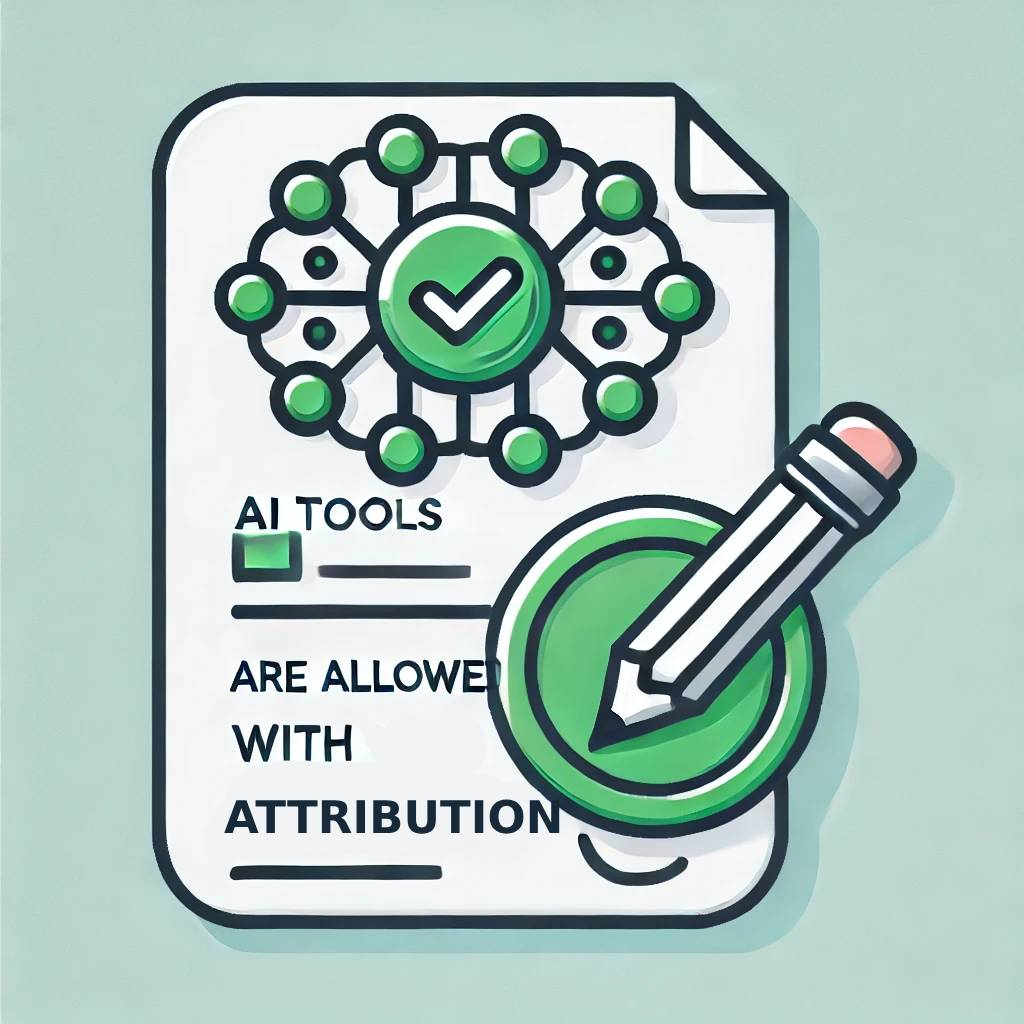
\includegraphics[width=1cm]{figs/Allowed_with_contributino.jpg}
    در این سوال قصد داریم به قابلیت دسته بندی بدون نمونه در مدل \lr{Clip} بپردازیم. بدین منظور از کتابخانه \href{https://github.com/mlfoundations/open_clip}{\lr{open-clip}} استفاده میکنیم.(۳۰ نمره)
    \begin{enumerate}
        \item ابتدا نسخه \lr{ConvNext-Base} را فراخوانی کنید. سپس از دیتاست \href{https://huggingface.co/datasets/maurice-fp/stanford-dogs}{\lr{Stanford-dogs}} (مجموعه آزمون)برای ارزیابی توانایی یادگیری بدون نمونه این مدل بهره بجویید. برای انتخاب قالب پرامپت متن مجاز هستید از یک قالب دلخواه استفاده کنید.
        \item چند قالب متن دیگر را به دلخواه امتحان کنید و نتایج آنها را مقایسه کنید. توجه داشته باشید، به علت تعداد بالای کلاس های مجموعه داده، انتخاب قالب های متفاوت برای کلاس های مختلف عملی به نظر نمیرسد.
        \item \lr{accuracy}، \lr{precision} ،\lr{recall} و \lr{F1} را به تفکیک کلاس گزارش کنید. کلاسی که بدترین \lr{F1} را دارد را اعلام کنید. سعی کنید برای این کلاس قالب های متفاوتی پیدا کنید تا عملکرد مدل درمورد آن کلاس بهبود یابد. نتایج را مقایسه کنید.
        \item برای هر کلاس یک جاگذاری قابل آموزش تعریف کنید و به کمک گرادیان کاهشی آنرا آموزش دهید(مجموعه آموزش). سپس  دقت را روی مجموعه آزمون محاسبه و گزارش کنید.
        \item رمزگذار متن را کنار بگذارید. رمزگذار تصویر را منجمد کرده و یک لایه تمام متصل اضافه کنید. لایه اضافه شده را آموزش دهید(مجموعه آموزش). سپس  دقت را روی مجموعه آزمون محاسبه و گزارش کنید.
        \item اینبار مدل \lr{ConvNext-XXLarge} را فراخوانی کرده و آزمایشهای قسمت الف و ب را با آن تکرار کرده، نتایج را مقایسه کنید.  
    \end{enumerate}
    
    \textcolor{red}{\textbf{توجه: برای گزارش این سوال نتایج را مقایسه، تحلیل و سپس توجیه کنید.}}
    
    \item 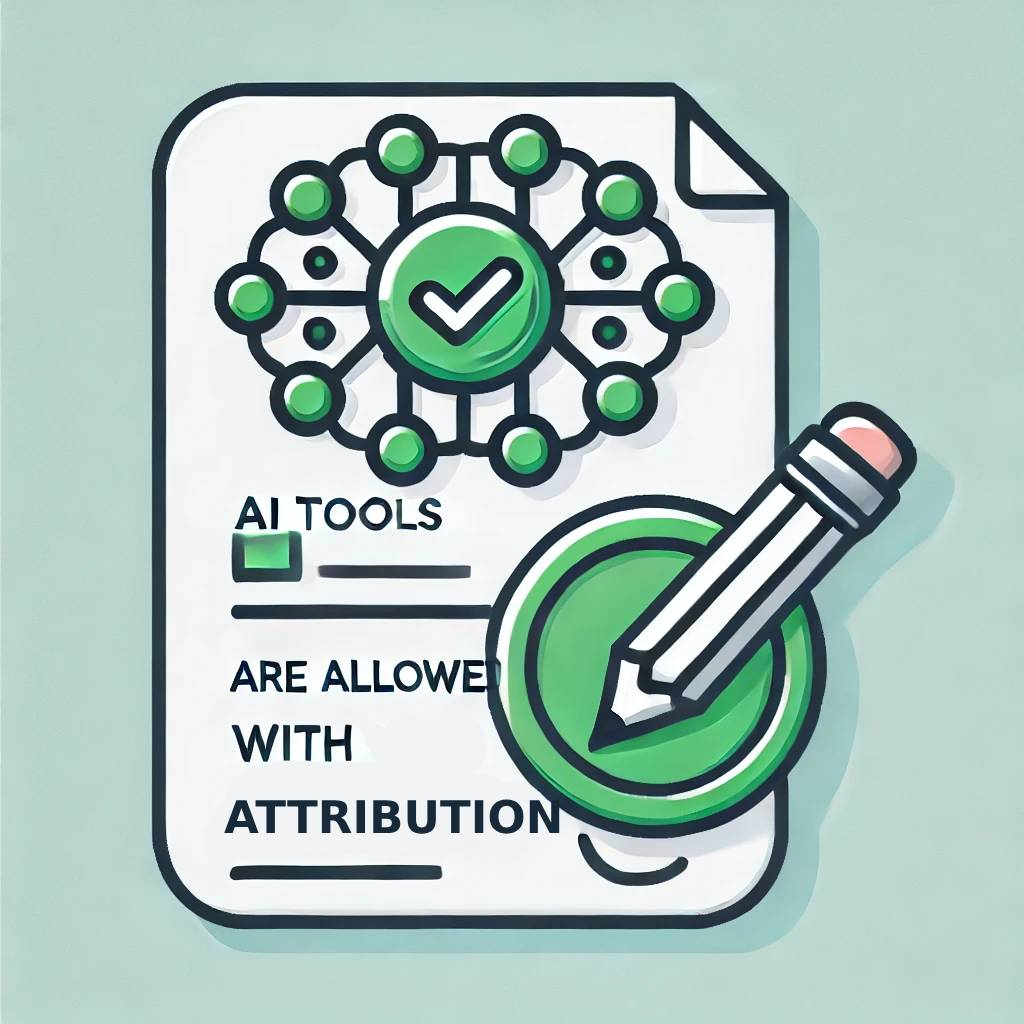
\includegraphics[width=1cm]{figs/Allowed_with_contributino.jpg}
     در این سوال قصد داریم با استفاده از یک مدل زبانی فارسی با \lr{soft prompting}  آشنا شده و سپس به روش‌هایی از \lr{Reasoning} بپردازیم. قسمت های مشخص شده در نوت بوک \lr{LLM.ipynb} را تکمیل کنید(۲۰ نمره).

     \item 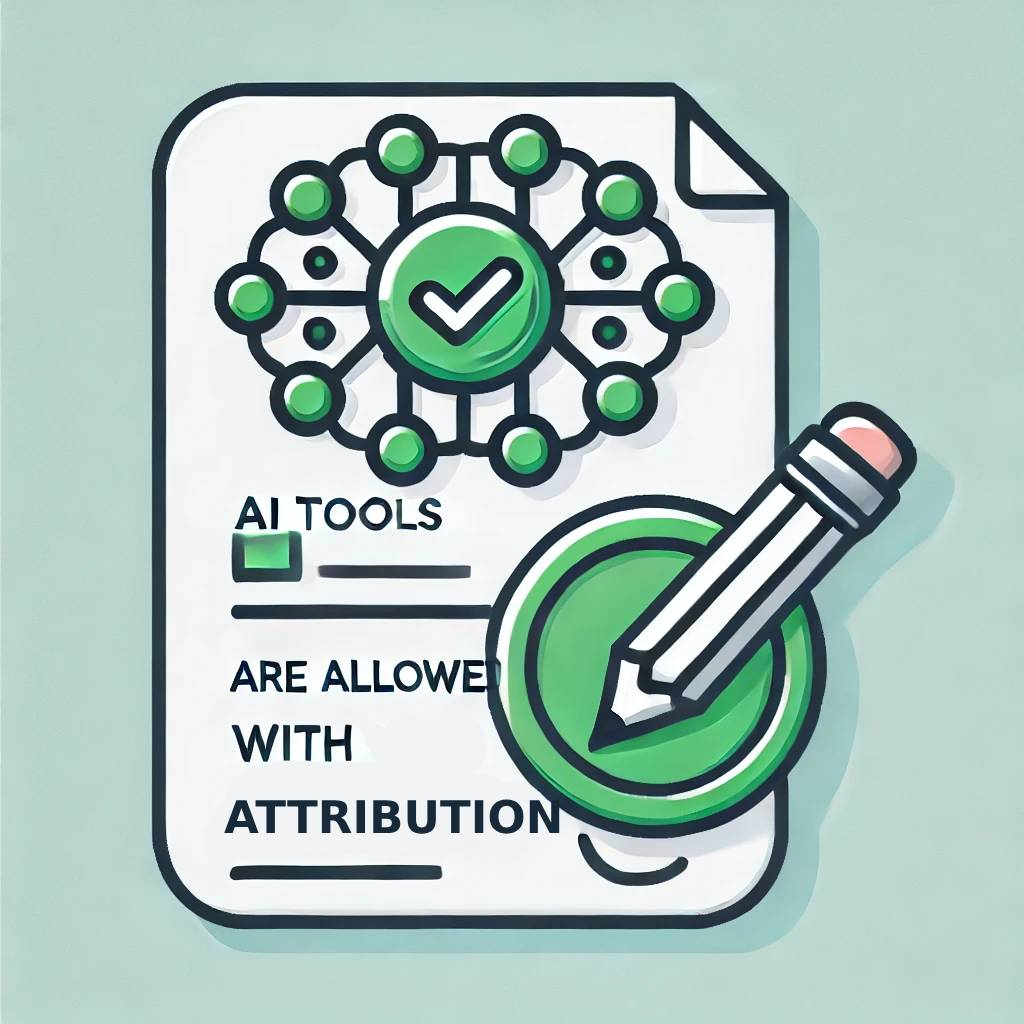
\includegraphics[width=1cm]{figs/Allowed_with_contributino.jpg}
     در این تمرین با استفاده از کتابخانه‌های  \lr{HuggingFace} و \lr{PEFT}، یک مدل \lr{Vision Transformer (ViT)} را روی دیتاست \lr{Food101} آموزش خواهید داد. هدف اصلی استفاده از روش \lr{Low-Rank Adaptation (LoRA)} برای آموزش مؤثرتر و کم‌هزینه‌تر مدل است. لطفا نوتبوک \lr{peft\_lora.ipynb} را کامل کنید(۲۰ نمره).

     \begin{itemize}
         \item داده‌ها را بارگذاری و آماده‌سازی کنید (از دیتاست \lr{food101} استفاده شده است).
         \item     مدل \lr{ViT} را از \lr{HuggingFace} بارگیری کنید.
        \item     با استفاده از \lr{PEFT} و \lr{LoRA}، بخش‌هایی از مدل را قابل آموزش قرار دهید.
        \item     مدل را با استفاده از \lr{Trainer} آموزش دهید.
        \item     در پایان، از مدل آموزش‌دیده برای پیش‌بینی تصویر جدید استفاده کنید.
    
     \end{itemize}
    


\end{enumerate}



\end{document}


